\documentclass[9pt,twocolumn,twoside]{pnas-new}

\usepackage{pnas-2025-compat}
\articletype{EARTH, ATMOSPHERIC, AND PLANETARY SCIENCES}
\templatetype{pnasresearcharticle}

% Use descriptive headings without numeric or alphabetic prefixes.
\setcounter{secnumdepth}{0}

% Match the class-specific Materials and Methods heading to the regular
% unnumbered PNAS section-heading typography.
\makeatletter
\titleformat{\matmethods@section}
  {\large\sffamily\bfseries}
  {}
  {0em}
  {#1}
  []
\makeatother

\usepackage{siunitx}

\graphicspath{{../figures/}}

\newcommand{\coTwo}{CO$_2$}
\newcommand{\todo}[1]{\textbf{[TODO: #1]}}

\begin{document}

\title{End-to-End Uncertainty Quantification of Geologic \coTwo{} Storage in Faulted Reservoirs}

\author[a,b]{Shaowen Mao}
\author[c]{Llu\'{\i}s Sal\'o-Salgado}
\author[d]{Hannah Lu}
\author[e]{Patricia Ascanio-Pellon}
\author[e]{Christie M. Rogers}
\author[e]{Nathan W. Harkins}
\author[e]{Rodrick D. Myers}
\author[e]{Lisa Lun}
\author[a,b,1]{Ruben Juanes}

\affil[a]{Department of Civil and Environmental Engineering, Massachusetts Institute of Technology, 77 Massachusetts Avenue, Cambridge, Massachusetts 02139, USA}
\affil[b]{Earth Resources Laboratory, Department of Earth, Atmospheric and Planetary Sciences, Massachusetts Institute of Technology, 77 Massachusetts Avenue, Cambridge, Massachusetts 02139, USA}
\affil[c]{Department of Earth, Environmental, and Planetary Sciences, University of Tennessee, Knoxville, TN, USA}
\affil[d]{The Oden Institute for Computational Engineering and Sciences, The University of Texas at Austin, Austin, TX, USA}
\affil[e]{ExxonMobil Technology and Engineering Company, Spring, TX, USA}

\leadauthor{Mao}

% Replace the final sentence with the principal quantitative finding after the
% Phase-1 and targeted-enrichment analyses are complete.
\significancestatement{Faults are commonly represented by one effective property field even though their internal architecture is unresolved. We propagate uncertainty from fault--seal geology through stochastic three-dimensional fault-core properties to field-scale carbon dioxide migration and containment. Repeated full-fault realizations test whether a representative fault preserves the reservoir-scale conclusion across 162 prescribed geologies. This design separates broad geologic controls from realization-to-realization variability and identifies where ensemble modeling and additional fault characterization are most valuable for storage assessment.}

\authorcontributions{\todo{Assign author contributions using the final PNAS contribution taxonomy.}}
\authordeclaration{\todo{Add the final competing-interest declaration for all authors.}}
\correspondingauthor{\textsuperscript{1}To whom correspondence should be addressed: Ruben Juanes. Email: juanes@mit.edu}

\keywords{geologic carbon storage $|$ faults $|$ uncertainty quantification $|$ multiphase flow $|$ reservoir simulation}

\begin{abstract}
Faults can either impede or transmit injected \coTwo{}, but unresolved fault-core structure makes their influence on storage security difficult to assess. Most field-scale models use one representative fault, implicitly assuming that local stochastic variability does not alter the containment conclusion. We develop an end-to-end framework to test that assumption across a prescribed fault--seal geologic design space. For each of 162 geologic scenarios and six throw windows, PREDICT generates 2,000 stochastic three-dimensional fault-core realizations. Physics-based upscaling provides joint permeability, porosity, capillary-pressure, and relative-permeability properties, which are assembled into spatially heterogeneous full-fault fields. Phase 1 contains 12 conditionally independent full-fault realizations per geology for conditional uncertainty analysis, together with separate representative-medoid and low/high-state benchmarks. High-performance simulations of a roughly two-million-cell offshore Texas model track \coTwo{} retention, fault and top-seal entry, upward migration, and phase partitioning for 1,000 years. We use the balanced ensemble to identify geologic controls and quantify within-geology stochastic variability, then enrich selected geologies where initial realizations indicate mixed containment outcomes. \todo{Insert the dominant geologic effect, the frequency and magnitude of mixed outcomes, and the representative-fault performance.} The analysis determines when a representative fault is adequate and when stochastic fault-core ensembles are needed for reliable storage assessment.
\end{abstract}

\dates{This manuscript was compiled on \today}
\doi{10.1073/pnas.XXXXXXXXXX}

\maketitle
\thispagestyle{firststyle}
\ifthenelse{\boolean{shortarticle}}{\ifthenelse{\boolean{singlecolumn}}{\abscontentformatted}{\abscontent}}{}

% Keep three introductory paragraphs beside the first-page significance box,
% then restore the standard two-column width at paragraph four.
\firstpage{4}

% PNAS omits an explicit Introduction heading for research articles.
% PNAS research reports begin directly, without an explicit Introduction
% heading. Keep this file to four principal paragraphs so the first-page column
% transition controlled by \firstpage{4} remains predictable.

Climate-scale deployment of geologic carbon storage requires confidence that
injected \coTwo{} remains contained over operational and post-injection time
scales. Faults are central to that assessment because they can impede flow,
transmit fluids along their planes, or connect otherwise separated units.
Their influence cannot always be reduced to a binary seal-or-conduit label:
the same fault--seal setting can support different migration pathways as its
unresolved internal structure changes. Reliable site assessment therefore
requires knowing not only the expected fault behavior, but also whether
unresolved fault structure can change the containment conclusion.

This requirement creates a multiscale problem. Field characterization
constrains aspects of stratigraphy, fault throw, and burial history, whereas
the local arrangement and continuity of fault-core materials remain
unresolved. That architecture controls anisotropic permeability, porosity,
capillary entry, and phase mobility, while field-scale simulations represent
the fault with much coarser elements. A single representative property field
implicitly assumes that unresolved local variability does not materially
alter the reservoir-scale prediction. That assumption has not been tested
systematically across a broad fault--seal geologic design space.

Stochastic fault-property modeling and multiphase upscaling begin to bridge
this scale gap. PREDICT links local stratigraphy and fault throw to
distributions of three-dimensional anisotropic fault permeability
\cite{SaloSalgado2023}. Pettersson et al.\ upscale stochastic fault properties,
preserve dependence among flow functions, and propagate them to field-scale
leakage distributions, while identifying fully three-dimensional fault
variation as an unresolved limitation \cite{Pettersson2025}. Field-scale
studies further demonstrate that fault representation can influence modeled
\coTwo{} migration and storage-security metrics
\cite{SaloSalgado2025,Lu2025}. What remains unclear is how the importance of
stochastic fault-core structure changes across fault--seal geologies and when
one representative fault gives a misleading reservoir-scale prediction.

Here, we use an end-to-end uncertainty-quantification framework to determine
(i) which characteristics of the fault--seal system control \coTwo{} migration
and containment, (ii) in which geologic settings stochastic fault-core
realizations produce different containment outcomes, and (iii) when a
representative fault is sufficient for storage assessment. We connect
stochastic local three-dimensional fault-core modeling, physics-based
multiphase upscaling, conditionally independent full-fault property sampling,
and field-scale simulation across 162 prescribed geologic scenarios. A
balanced initial ensemble supports comparisons across all geologies, while
targeted enrichment resolves conditional outcome distributions where the
initial realizations indicate mixed behavior.


% !TEX root = ../manuscript.tex

\section{End-to-end uncertainty quantification workflow}

The framework connects uncertainties that are commonly treated in isolation:
fault--seal geology, unresolved fault-core architecture, spatially variable
full-fault properties, and field-scale \coTwo{} migration and containment
(Fig.~\ref{fig:end-to-end-workflow}). It has three linked components---local
fault-property modeling, full-fault property sampling, and field-scale storage
simulation. This hierarchy allows broad geologic effects to be distinguished
from residual stochastic variability conditional on a prescribed geology.

At the local scale, the 162 geologic scenarios specify structural and
stratigraphic conditions within six throw windows. For every geology--window
combination, PREDICT generates 2,000 stochastic three-dimensional fault-core
architectures and their joint anisotropic permeability. Exact realization
replay and physics-based upscaling then provide internally consistent
permeability, porosity, capillary-pressure, and relative-permeability
properties.

At the full-fault scale, selected local realizations populate six windows
along dip and 87 slices along strike. Phase 1 uses 12 conditionally independent
full-fault realizations per geology to characterize stochastic variability,
while a full-distribution medoid and coherent low- and high-state fields serve
as separate deterministic benchmarks. Reproducible manifests preserve the
selected realization, seed, code version, and property provenance for every
fault element.

At the field scale, JutulDarcy propagates these heterogeneous fault properties
through a roughly two-million-cell offshore Texas storage model over 1,000
years. The balanced ensemble identifies geologic controls and within-geology
variability in migration and containment, and targeted enrichment resolves
conditional outcome distributions for geologies that exhibit mixed behavior.
The study design and assumptions needed to interpret the ensemble are
summarized in Materials and Methods. Complete sampling, replay, upscaling,
simulation, validation, and analysis procedures are provided in the SI
Appendix.


\begin{figure*}[t!]
  \centering
  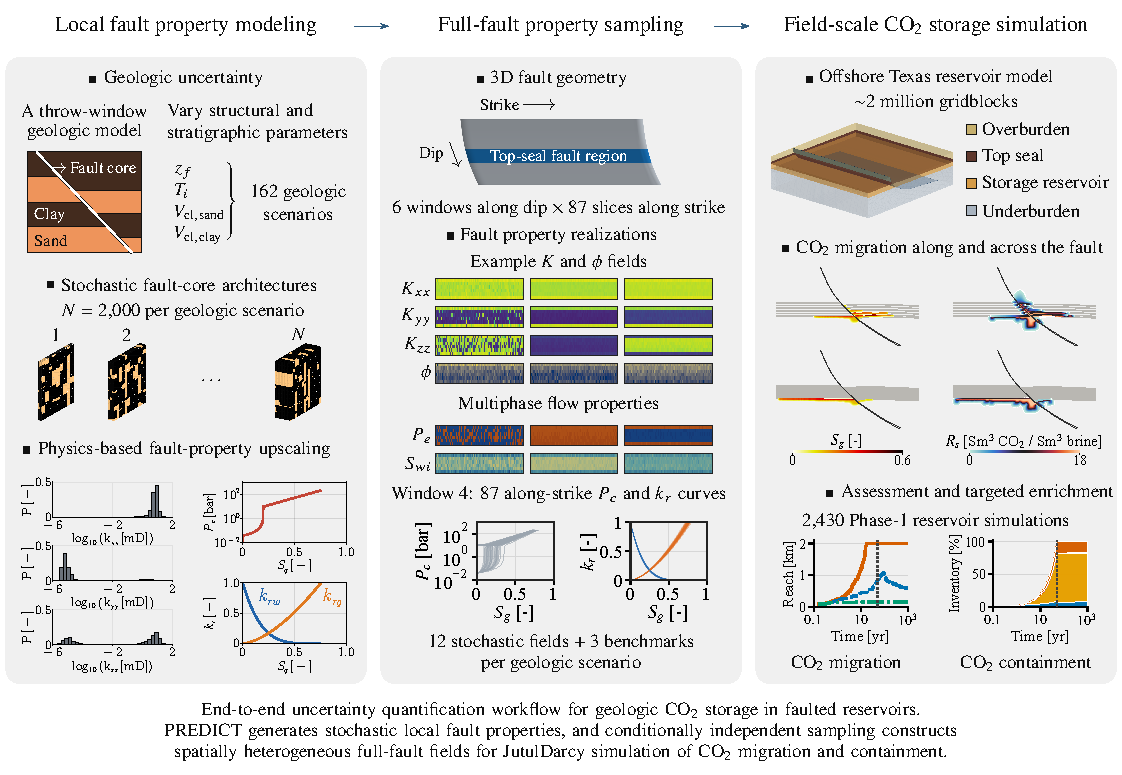
\includegraphics[width=\textwidth,trim=0 15mm 0 0,clip]{workflow/workflow_overview.pdf}
  \caption{End-to-end uncertainty quantification of \coTwo{} migration and
  containment in faulted reservoirs. PREDICT maps local fault--seal geology to
  stochastic three-dimensional fault-core properties; physics-based upscaling
  and conditionally independent full-fault sampling generate spatially
  heterogeneous $\mathbf{K}$, $\phi$, $P_c$, and $k_r$ fields; and JutulDarcy
  propagates those fields through field-scale storage simulations. Phase 1
  evaluates all 162 prescribed geologies with 12 stochastic fields and three
  separate benchmark fields per geology. Reservoir outcomes guide targeted
  enrichment of geologies with mixed behavior.}
  \label{fig:end-to-end-workflow}
\end{figure*}

% !TEX root = ../manuscript.tex

\section{Results}

The analysis is organized around the reservoir-scale questions enabled by the
framework. We first identify geologic controls on typical migration and
containment, then quantify realization-to-realization variability within each
geology. Targeted enrichment resolves conditional outcome distributions in
geologies with mixed behavior, and the deterministic benchmarks test when a
representative fault preserves the ensemble-level conclusion.

\subsection{Geologic controls on typical migration and containment}

\todo{Lead with one primary containment quantity and one primary migration
quantity. Report design-based main effects and selected interactions for
thickness structure, faulting depth, sand-layer clay volume fraction, and
clay-layer clay volume fraction. For zero-inflated quantities, separate the
occurrence of fault or top-seal entry from the magnitude after entry. Report
standardized effects and uncertainty intervals, and describe these as effects
over the prescribed, unweighted geologic design space rather than as
field-calibrated probabilities.}

\subsection{Within-geology variability from stochastic fault-core structure}

\todo{For every geology, report robust conditional spread, outcome-class
frequencies, and whether the 12 realizations cross a physically defined
containment threshold. Classify geologies using predefined categories such as
consistently contained, mixed containment outcomes, and consistently
migrating. Support this classification with the balanced design-based
decomposition of between-geology and average within-geology variability.}

\subsection{Conditional outcome distributions in enriched geologies}

\todo{Describe the prespecified enrichment criteria and report empirical CDFs,
quantiles with bootstrap intervals, and outcome frequencies with binomial
intervals for the selected geologies. Use newly added realizations to confirm,
rather than merely redisplay, realization sensitivity first observed in Phase
1. Include consistently contained and consistently migrating controls so the
selection cannot be interpreted as focusing only on anomalous cases.}

\subsection{Performance of representative-fault benchmarks}

\todo{Compare each full-distribution-medoid result with the conditional
stochastic distribution. Report its difference from the stochastic median,
its empirical CDF position, and its agreement with the majority outcome class.
Treat the low/high fields as unweighted stress benchmarks rather than bounds,
percentiles, or probabilistic realizations. Emphasize the conditions under
which a representative fault is adequate and those under which it gives a
misleading single answer.}

% !TEX root = ../manuscript.tex

\section{Discussion}

\todo{Open with three quantitative findings: the dominant geologic controls,
the geologic settings in which stochastic realizations change the containment
class, and the observed performance of the representative-fault benchmark.}

\subsection{Why end-to-end uncertainty propagation is needed}

The contribution is not simply the connection of several numerical tools.
The framework preserves the chain from fault--seal geology to plausible local
fault-core architectures, physically consistent
$(\mathbf{K},\phi,P_c,k_r)$ properties, full-fault fields, and
reservoir-scale outcome distributions. This common chain permits direct
comparison of broad geologic effects, residual within-geology stochastic
effects, and representative versus ensemble predictions without replacing
joint fault properties by independently averaged components.

\subsection{When is stochastic fault modeling needed?}

The required level of fault representation should be tied to the stability of
the storage conclusion. Where stochastic realizations are consistently
contained and the medoid agrees with the ensemble, a representative fault may
be adequate for initial assessment. Mixed containment outcomes indicate that
an ensemble is needed and that additional fault characterization or monitoring
has greater value. Where all realizations migrate substantially, further
sampling may refine the magnitude without changing the broad site or
injection-management conclusion. \todo{Replace these conditional statements
with a compact result-supported guide after the enriched simulations are
analyzed.}

\subsection{Relation to previous uncertainty-propagation studies}

Pettersson et al.\ demonstrate stochastic upscaling, preserve dependence among
multiphase fault properties, and propagate those properties to field-scale
leakage distributions using a one-dimensional fine-scale fault description
\cite{Pettersson2025}. Our framework extends the scientific question to a
broad fault--seal design space and a spatially variable three-dimensional
fault: where does additional stochastic detail change the storage conclusion,
and where does it not? This distinction is more useful than assuming either
that one representative fault is universally sufficient or that every site
requires the same ensemble size.

These findings should be interpreted within the scope of the modeled design.
The 162 scenarios span a balanced geologic design space but do not carry
field-calibrated occurrence probabilities. PREDICT realizations are
model-based samples conditional on the prescribed geology, not observations
of the real fault. Full-fault stochastic fields assume conditional
independence after conditioning on geology and throw window because available
data do not constrain a coarse-scale spatial covariance model; they therefore
omit uncertainty in unresolved large-scale fault continuity. The enriched
ensembles support common and moderately uncommon outcomes, not precise
rare-event probabilities. Results also remain conditional on the reservoir
model, constitutive assumptions, injection scenario, and exclusion of
geomechanical reactivation.

% !TEX root = ../manuscript.tex

\section{Conclusions}

This study establishes an end-to-end framework for propagating uncertainty
from fault--seal geology and unresolved fault-core architecture to
field-scale \coTwo{} migration and containment. By separating variation
across prescribed geologies from stochastic variation within each geology,
the framework directly tests whether one representative fault preserves the
storage conclusion or conceals consequential alternative outcomes.

\todo{Replace this paragraph with the principal quantitative conclusions:
the dominant geologic controls, the frequency and magnitude of mixed
containment outcomes, the contribution of within-geology variability, and
the performance of the representative-fault benchmark.}

The required level of fault representation is not universal. A representative
fault may be sufficient where the containment conclusion is stable across
realizations, whereas mixed outcomes motivate stochastic ensembles,
additional fault characterization, or targeted monitoring. The framework
therefore provides both a reproducible uncertainty-propagation tool and a
practical basis for deciding where additional fault detail is consequential
for storage assessment.


% PNAS places the concise Materials and Methods summary after the findings;
% complete procedures are consolidated in the separately compiled SI Appendix.
% The class applies \small to this block by default. Restore the main-text
% font and baseline spacing so the Methods typography matches the article.
\matmethods{{\normalsize% !TEX root = ../manuscript.tex

The study uses a balanced, unweighted design of 162 prescribed fault--seal
geologies. Each geology is represented by six throw windows, and PREDICT
generates 2,000 joint anisotropic-permeability realizations for every
geology--window combination. Selected realizations are replayed and upscaled
to internally consistent permeability, porosity, capillary-pressure, and
relative-permeability properties. The complete geologic design, PREDICT
generation rules, convergence assessment, replay procedure, and property
upscaling calculations are provided in the SI Appendix.

For each geology, Phase 1 contains 12 stochastic full-fault realizations plus
three separate deterministic benchmarks: a full-distribution medoid and
coherent low- and high-state fields. Each stochastic field contains one draw
for every combination of six windows and 87 along-strike slices. Draws are
uniform with replacement and conditionally independent after conditioning on
geology and throw window; this construction avoids imposing an unsupported
cross-window or along-strike covariance model and does not assert that real
faults are spatially independent. Only the 12 stochastic fields enter
probabilistic and variance-based analyses. The deterministic fields diagnose
representative and stress behavior and are not interpreted as probabilities,
bounds, or percentiles. Sampling algorithms, state construction, stable seed
generation, provenance manifests, and validation tests are documented in the
SI Appendix.

JutulDarcy propagates the heterogeneous full-fault properties through a
roughly two-million-cell offshore Texas storage model for 1,000 years. Primary
responses quantify top-seal entry and maximum upward migration; secondary
responses quantify storage-reservoir retention, fault entry, and dissolved
and free-phase partitioning. Geologic effects and average within-geology
variability are estimated from the common 12-realization balanced ensemble.
Prespecified outcome criteria identify geologies for additional independent
realizations, while enriched cases remain excluded from the balanced global
variance decomposition. Complete model settings, spatial definitions,
quantities of interest, statistical estimators, enrichment rules, and
reservoir-input consistency checks are provided in the SI Appendix.
}}
\showmatmethods{}

\dataavail{The PREDICT source code and reproducible analysis workflow are maintained at \url{https://github.com/ShaowenMao/predict_shaowen}. \todo{Deposit the submitted software version and derived data in archival repositories; add persistent identifiers, licenses, dataset citations, and any access conditions.}}

\acknow{\todo{Add funding, computing resources, and technical contributions.}}
\showacknow{}

\bibliography{references}

\end{document}
